% book example for classicthesis.sty
\documentclass[
  % Replace twoside with oneside if you are printing your thesis on a single side
  % of the paper, or for viewing on screen.
  oneside,
  %twoside,
  11pt, a4paper,
  footinclude=true,
  headinclude=true,
  cleardoublepage=empty
]{scrbook}

\usepackage{lipsum}
\usepackage[linedheaders,parts,pdfspacing]{classicthesis}
\usepackage{amsmath}
\usepackage{amsthm}
\usepackage{acronym}
\usepackage{listings}

\renewcommand\lstlistingname{List of Listings}
\renewcommand\lstlistlistingname{List of Listings}

\title{CS488 Ray Tracer Final Project}
\author{Sekhar Bhattacharya}

\begin{document}

\maketitle

% Front Matter
%*******************************************************
% Table of Contents
%*******************************************************
\pdfbookmark[1]{\contentsname}{tableofcontents}
\addcontentsline{toc}{chapter}{Table of Contents}

\setcounter{tocdepth}{2} % <-- 2 includes up to subsections in the ToC
\setcounter{secnumdepth}{3} % <-- 3 numbers up to subsubsections

\tableofcontents 

%*******************************************************
% List of Figures and of the Tables
%*******************************************************

%*******************************************************
% List of Figures
%*******************************************************    
\pdfbookmark[1]{\listfigurename}{lof}
\addcontentsline{toc}{chapter}{\listfigurename}
\listoffigures

%*******************************************************
% List of Tables
%*******************************************************
%\pdfbookmark[1]{\listtablename}{lot}
%\addcontentsline{toc}{chapter}{\listtablename}
%\listoftables
  
%*******************************************************
% List of Listings
%******************************************************* 
\pdfbookmark[1]{\lstlistlistingname}{lol}
\addcontentsline{toc}{chapter}{\lstlistlistingname}
\lstlistoflistings
   
%*******************************************************
% Acronyms
%*******************************************************
%\pdfbookmark[1]{Acronyms}{acronyms}
%\chapter*{Acronyms}
%\begin{acronym}[UML]
%    \acro{DRY}{Don't Repeat Yourself}
%    \acro{API}{Application Programming Interface}
%    \acro{UML}{Unified Modeling Language}
%\end{acronym} 

%*******************************************************
% Acknowledgments
%*******************************************************
\pdfbookmark[1]{Acknowledgements}{acknowledgements}
\addcontentsline{toc}{chapter}{Aknowledgements}
\chapter*{Acknowledgements}

I acknowledge that I have heavily referenced code from \cite{9_perlin_2002} as 
well as \cite{7_kora_2007} in order to complete the Perlin noise objective. The 
reference especially helped me understand how the Perlin noise function can be
used to create natural looking textures.



% Body
%*******************************************************
% Introduction
%*******************************************************
\pdfbookmark[1]{Introduction}{introduction}
\chapter{Introduction}

\section{Purpose}
The purpose of this project is to design and implement a functional ray tracer
satisfying the ten objectives listed below. The ten objectives are of reasonable
complexity and are functionalities which I believe are necessary for a 
reasonably complex ray tracer to posses.

\section{Statement}
I will attempt to build a reasonably complex ray tracer able to generate
photorealistic images of complex scenes that satisfy the ten objectives listed
below. I am also interested in implementing extra functionality such as parallel
ray tracing, uniform space subdivision, caustics using illumination map and
motion blur. I will generate scenes that display the functionality of each of
the objectives listed below and if time permits I will also attempt to satisfy
any extra objectives. As a note, I have implemented mirror reflections as part
of assignment four and so have not included it as an objective for ths project.

I find the topic of ray tracing to be very interesting to me and I have spent
considerable amount of time reading the seminal literature related to ray
tracing techniques. The challenge for me will be to implement these techniques
in an efficient manner while generating high quality images. Soft shadows,
glossy reflection and anti-aliasing (three of the techniques I wish to implement
for this project) are all techniques that increase the time it takes to produce
a ray traced image and it will be quite a challenge to implement these
techniques efficiently.

I hope that at the completion of this project I will learn many of the important
algorithms and techniques used in ray tracing as well as learning new and better
methods of efficient programming. I hope to also keep working on this project
even after completing this course and continue to implement other modern ray
tracing techniques.

\section{Objectives}
Below is a list of the objectives for this project in the order in which they
were completed. 

\begin{itemize}
  \item Extra Primitives
  \item Constructive Solid Geometry
  \item Anti-Aliasing
  \item Soft Shadows
  \item Texture Mapping
  \item Bump Mapping
  \item Phong Shading
  \item Refraction
  \item Glossy Reflection
  \item Perlin Noise
\end{itemize}

The two objectives I had stuggled with the most during the
project was bump mapping and perlin noise. Although the concept of bump mapping
is similar to that of texture mapping (which I had found relatively simple to
implement), I struggled with understangin the mathematics behind the
implementation of bump mapping. For Perlin noise, I was able to implement the
relatively straight-forward noise function but struggled to understand how to
use the noise function in a way to generate meaningful textures.

%*******************************************************
% Manual
%*******************************************************
\pdfbookmark[1]{Manual}{manual}
\chapter{Manual}

\section{Usage}
Running the ray tracer is very simple. Assuming the scene is specified by a file
named \verb|scene.lua|, then to run the ray tracer on the specified scene file
the following command shall be entered into the shell:
\begin{lstlisting}
    ./rt scene.lua
\end{lstlisting}
An image file will be produced in the same directory with the filename specified
in the  \verb|scene.lua| file. There will be no user interaction while the ray
tracer executable is running. The program will, however, display a progress bar.

There are no other command line options available for the executable. However,
optional parameters can be specified in the Lua scene file which will be
described in the next section.

\section{Modelling Language Extensions}
The LUA modelling language was extended to support many of the objectives that
were implemented for this project. Below is a summary of the changes made to old
commands as well as new commands that were added to the language for each of the
objectives implemented for this project.

\subsection*{Render Command}
The render command was extended to accept optional parameters to support
multi-threading, mirror reflections, anti-aliasing, soft shadows, and glossy
reflections and background images:
\begin{lstlisting}
  gr.render(<scene_root_node>, <filename>, <width>, <height>, <eye>, <view>,
  <up>, <fov>, <ambient>, <lights>, <threads> = 1, <recurse_level> = 0,
  <aa_samples> = 1, <shadow_samples> = 1, <glossy_samples> = 1,
  <background_filename> = null)
\end{lstlisting}
The \verb|<threads>| option is used to specify the number of threads used by the
ray tracer. The default is one thread.

The \verb|<recurse_level>| option specifies the maximum number of times that the
\verb|a4_trace_ray| function is called recursively. The default for this option
is zero in which case mirror reflections and refractions will not be rendered.

The \verb|<aa_samples>| option specifies the number of rays that are cast for each
pixel in order to perform anti-aliasing. The default is one ray per pixel.

The \verb|<shadow_samples>| option specifies the number of shadow rays that are
cast for each pixel in order to perform soft shadow rendering. The default is
one shadow ray per pixel.

The \verb|<glossy_samples>| option specifies the number of reflection rays that
are cast for each pixel in order to perform glossy reflection rendering. The
default is one reflection ray per pixel.

The \verb|<background_filename>| option specifies the filename of the image to
use as the background for the scene. The default is a null value meaning no
background image will be used.

\subsection*{Extra Primitives}
The following commands were added to the language in order to support rendering
of extra primitives.
\begin{itemize}
  \item \verb|gr.cone(<name>)|
  \item \verb|gr.cylinder(<name>)|
  \item \verb|gr.disc(<name>)|
  \item \verb|gr.plane(<name>)|
  \item \verb|gr.torus(<name>)|
\end{itemize}

\subsection*{Constructive Solid Geometry}
The following commands were added to the language in order to support rendering
of constructive solid geometry objects.
\begin{itemize}
  \item \verb|gr.csg_union(<name>, <geometry_node>, <geometry_node>)|
  \item \verb|gr.csg_intersection(<name>, <geometry_node>, <geometry_node>)|
  \item \verb|gr.csg_difference(<name>, <geometry_node>, <geometry_node>)|
\end{itemize}

\subsection*{Anti-Aliasing}
See the modifications made to \verb|gr.render| command above in order to support
anti-aliasing in the modelling language.

\subsection*{Soft Shadows}
The following command was added to the language to create area lights that are
used for the soft shadow computations:
\begin{lstlisting}
  gr.disc_light(<position>, <colour>, <attenuation>, <normal>, <radius>)
\end{lstlisting}
The command is a modification of the \verb|gr.light| command with two new
parameters added. The \verb|<normal>| parameter specifies the normal of the disc
light source and the \verb|<radius>| parameter specifies the radius of the disc
light source.

\subsection*{Texture Mapping}
The following command was added to the language to apply a texture image file
to the specified \verb|node|:
\begin{lstlisting}
  node:set_texture(<filename>)
\end{lstlisting}
The \verb|node| object must have had a material applied before using this
command via the \verb|set_material| command.

\subsection*{Bump Mapping}
The following command was added to the language to apply a bump map image file
to the specified \verb|node|:
\begin{lstlisting}
  node:set_bumpmap(<filename>)
\end{lstlisting}
The \verb|node| object must have had a material applied before using this
command via the \verb|set_material| command.

\subsection*{Phong Shading}
The following command is used to construct a mesh with a set of vertices and a
set of faces that contain indices into the vertex list:
\begin{lstlisting}
  gr.tri_mesh(<name>, <verts>, <faces>)
\end{lstlisting}
This command differs from the \verb|gr.mesh| command in that it subdivides the
faces into triangles as well as generating per vertex normals on instantiation.

\subsection*{Refraction}
The \verb|gr.material| command was extended as follows:
\begin{lstlisting}
  gr.material(<diffuse>, <specular>, <shininess>, <ni> = 0)
\end{lstlisting}
The optional \verb|<ni>| parameter was added to specify the index of refraction
of the material. The default value is zero which indicates that the material is
not refractive.

\subsection*{Glossy Reflection}
See the modifications made to the \verb|gr.render| command above in order to
support anti-aliasing.

\subsection*{Perlin Noise}
The following command was added to the language to apply a procedurally
generated texture using Perlin noise to the specified \verb|node|:
\begin{lstlisting}
  node:set_perlin(<type>)
\end{lstlisting}
The \verb|<type>| option specifies which procedural texture to apply to the
node. The \verb|node| object must have had a material applied before using this
command via the \verb|set_material| command.


%*******************************************************
% Code Organization
%*******************************************************
\pdfbookmark[1]{Code Organization}{code organization}
\chapter{Code Organization}

\section{Directory Structure}
All code and data files are located in the \verb|~/cs488/handin/A5| directory.

A \verb|README| file is located in the above directory detailing how to build
and use the ray tracer. It also lists all the objectives implemented for the
project.

\verb|*.cpp| and \verb|*.hpp| source files are located in the \verb|src| 
subdirectory. The \verb|Makefile| is in this subdirectory as well.

The \verb|data| subdirectory contains all the LUA scripts used to demonstrate
the objectives implemented for the project. It also contains a \verb|textures|,
\verb|bumps|, \verb|backgrounds| and \verb|objs| subdirectories which contain
the texture images, the bump maps, the background images and the mesh
definitions respectively. The textures, bump maps and background images must be
in PNG format. The mesh definition files must be in the OBJ format.

\section{Code Map}
Below is a list of all the source files in the project and brief description of
their purpose.

\subsection*{a4.cpp, a4.hpp}
This is the where the core of the ray tracer is contained. This file includes
the recursive \verb|a4_trace_ray| function as well as functions to generate
reflection and refaction rays. It also contains code for thread creation and the
\verb|a4_lighting| function which applies the Lambertion lighting model to each
pixel.

\subsection*{algebra.cpp, algebra.hpp}
These files contains \verb|Point2D|, \verb|Point3D|, \verb|Vector2D|,
\verb|Vector3D|, \verb|Matrix4x4| and \verb|Colour| classes as well as 
structures to represent \verb|Rays| and \verb|Intersections|.

\subsection*{image.cpp, image.hpp}
These files contains a class to load, save and manipulate PNG image files.

\subsection*{light.cpp, light.hpp}
These files contains the \verb|Light| class to represent point lights and the
\verb|DiscLight| class to represent area lights.

\subsection*{lua488.hpp}
This file just includes some of the Lua headers.

\subsection*{main.cpp}
This is the main entry point of the program. It just initializes the Lua
environment and hands off execution to the Lua interpreter which begins
interpreting the given Lua scene script.

\subsection*{material.cpp, material.hpp}
These files contain the \verb|Material| and \verb|PhongMaterial| class which
represents a material. The \verb|PhongMaterial| class was extended in order to
support textures, bump maps and index of refraction attributes.

\subsection*{mesh.cpp, mesh.hpp}
These files contain the implementation of the \verb|Mesh| class which holds a
list of vertices and faces. The \verb|Mesh| class is a sub-class of the
\verb|Primitive| class which means it must implement the \verb|intersection|
method. A new class was added, \verb|TriMesh|, which is a sub-class of 
\verb|Mesh| which subdivides a mesh's face list into triangles and then
generates and stores per-vertex normals on instantiation.

\subsection*{perlin.cpp, perlin.hpp}
These files contain the \verb|Perlin| class which contains only static methods
that generate scaling factors (which follow a certain pattern depending on the
desired texture) that are used to modify the diffuse colour of a material.

\subsection*{polyroots.cpp, polyroots.hpp}
These files contain functions to solve quadratic, cubic and quartic polynomial
equations.

\subsection*{primitive.cpp, primitive.hpp}
These files contain a number of primitive classes described in the last section.
Listed below are the extra primitive classes that were added to this file:
\begin{itemize}
  \item \verb|Cone|
  \item \verb|Cylinder|
  \item \verb|Disc|
  \item \verb|Plane|
  \item \verb|Torus|
\end{itemize}
Each of these primitive classes implement the \verb|intersection| method.

\subsection*{scene.cpp, scene.hpp}
These files contain the \verb|SceneNode| class and it's sub-classes, most 
notably the \verb|GeometryNode| and \verb|ConstructiveSolidGeometryNode| 
classes. The \verb|SceneNode| class is used to construct a scene graph
containing a number of primitives and meshes.

\subsection*{scene\_lua.cpp, scene\_lua.hpp}
These files contain the implementation of the custom Lua commands used for the
modelling language. All new Lua commands and modifications of old commands were
added here.


%*******************************************************
% Implementation
%*******************************************************
\pdfbookmark[1]{Implementation}{implementation}
\chapter{Implementation}

This section will describe the implementation of each of the objectives
including specific algorithms and data structures used and changes made to the
Lua modelling language.

%*******************************************************
% Extra Primitives
%*******************************************************
\section{Extra Primitives}

This section will described how the \verb|intersection| method was
implemented for each of the extra primitives. As mentioned in the 
previous section, the primtive classes were added to the \verb|primitives.cpp| 
source file.

The \verb|intersection| method takes two parameters. The first parameter is a
\verb|Ray| object and the second parameter is an \verb|Intersection| object. The 
intersection object is modified by an intersection method when an intersection 
has occurred. The method returns true on intersection and false otherwise.

A ray can be represented by the equation $R = O + t\vec{D}$ where
O is the ray's origin and $\vec{D}$ is the ray's direction. The \verb|Ray| 
object contains the ray's origin and direction. The point, $R$, on the ray can 
be determined given the $t$ parameter. The intersection code aims to calculate 
the value of the $t$ parameter such that the point on the ray's line is the 
point of intersection on the primitive \cite{5_drakos_1997}. 

The \verb|Intersection| object is where the intersection details are
stored such as the point of intersection, the normal at the point of
intersection (used for lighting calculations), the material of the primitive
(used for lighting calculations), the texture coordinates (used in texture
mapping), and the tangent vectors (used in bump mapping). All intersection tests 
are done in the primtives' local coordinate system with unit sized primitives.

\subsection*{Cone}
The \verb|gr.cone(<name>)| Lua command is used to create a single-ended cone 
aligned along the $z$-axis with unit height, $h$.

The cone primitive is specified by the implicit equation $x^2 + y^2 = z^2, -h <
z < h$.

In order to determine the intersection of a ray with a cone the implicit
equation must be solved by substituting in the equation of the ray:
\begin{equation}
  (O_{x} + t\vec{D}_{x})^2 + (O_{y} + t\vec{D}_{y})^2 = \\
  (O_{z} + t\vec{D}_{z})^2
\end{equation}
This equation expands to:
\begin{equation}
\begin{split}
  (\vec{D}_{x}^2 + \vec{D}_{y}^2 - \vec{D}_{z}^2)t^2 + (2O_{x}\vec{D}_{x} + 
  2O_{y}\vec{D}_{y} - 2O_{z}\vec{D}_{z})t + \\
  (O_{x}^2 + O_{y}^2 - O_{z}^2) &= 0\label{cone2}
\end{split}
\end{equation}
The equation specified in~(\ref{cone2}) can be solved for $t$ using the
quadratic equation. If the value of $t$ cannot be determined or the if $t$ is
negative, indicating that the intersection point is behind the ray's origin,
then there is no intersection. If $t$ is positive then the ray intersects the
cone and the intersection point is checked to make sure that the inequality $-h
< z < h$ is satisfied.

The normal vector is calculated by the following equation:
\begin{equation}
  \vec{N} = \begin{bmatrix} 2Q_{x} & 2Q_{y} & -2Q_{z}
  \end{bmatrix}^{T}
\end{equation}
Where $Q$ is the intersection point. The equation is essentially calculating the
gradient of the intersection point over the surface of the cone.

\subsection*{Cylinder}
The \verb|gr.cylinder(<name>)| Lua command is used to create a cylinder aligned
along the $z$-axis with unit height, $h$, and unit radius, $r$.

The cylinder primitive is specified by the implicit equation $x^2 + y^2 = r^2 =
1, \frac{-h}{2} < z < \frac{h}{2}$.

Similar to the cone, the intersection of a ray with a cylinder can be determined
by solving a quadratic equation with the following coefficients:
\begin{equation}
\begin{split}
  a_{2} &= \vec{D}_{x}^2 + \vec{D}_{y}^2 \\
  a_{1} &= 2O_{x}\vec{D}_{x} + 2O_{y}\vec{D}_{y} \\
  a_{0} &= O_{x}^2 + O_{y}^2 - 1
\end{split}
\end{equation}
The intersection of the ray with the end caps of the cylinder are determined by
testing intersection between the ray and a disc which is described later in this
section.

The normal vector is easily determined. It is essentially the vector from the
origin to the intersection point with the $z$ coordinate set to zero.

\subsection*{Disc}
The \verb|gr.disc(<name>)| Lua command is used to create a disc centered at the
origin and lying on the $xy$-plane with unit radius, $r$.

To determine the intersection of the ray with the disc, it is a simple matter of
determining if the ray intersects the plane that contains the disc and then
validating whether the intersection point lies within the disc's area. The
ray-plane intersection is described later in this section. To validate whether
the intersection point is within the disc's area, the following inequality must
be satisfied:
\begin{equation}
  Q\cdot Q \leq r^2
\end{equation}
Where $Q$ is the vector from the origin to the intersection vector.

Since the disc lies on the $xy$-plane, the normal vector is simply \newline
$\begin{bmatrix} 0.0 & 0.0 & 1.0
\end{bmatrix}^{T}$.

\subsection*{Plane}
The \verb|gr.plane(<name>)| Lua command is used to create a bounded plane 
centered at the origin and lying on the $xz$-plane with unit height, $h$, and 
width, $w$. In reality, this primitive isn't really a plane but a rectangle
(unit square). However, it can be scaled to larger size. This primitive was
added since it provides a more efficient way for modelling walls or ground in a
scene.

A point $Q$ on a plane can be found with the following equation:
\begin{equation}
  \vec{N}\cdot (Q - P) = 0
\end{equation}
Where $\vec{N}$ is the normal vector of the plane and $P$ is a known point on
the plane. To solve for $Q$ we must substitute the equation of the ray into the
plane equation which we can then solve for $t$:
\begin{equation}
  t = \frac{\vec{N}\cdot (P - O)}{\vec{N}\cdot \vec{D}}
\end{equation}
Once the intersection point is found, it is a simple matter of determining if
the intersection point is within the bounded plane. This is done by simply
validating whether the $x$ and $z$ coordinates are within the unit square.

Since the bounded plane lies on the $xz$-plane, the normal vector is simply
$\begin{bmatrix} 0.0 & 1.0 & 0.0
\end{bmatrix}^{T}$.

\subsection*{Torus}
The \verb|gr.torus(<name>)| Lua command is used to create a torus centered at
the origin and lying on the $xy$-plane with unit major radius, $R$, and a minor 
radius, $r = 0.5$.

The implementation of the ray-torus intersection test is a bit more involved
than the other primitives as it requires solving a quartic equation. The
coefficients for this quartic equation are given by \cite{13_wagner_2004}:
\begin{equation}
\begin{split}
  a_{4} &= \vec{D}\cdot\vec{D} \\
  a_{3} &= 4(\vec{D}\cdot\vec{D})(\vec{O}\cdot\vec{D}) \\
  a_{2} &= 4(\vec{O}\cdot\vec{D})^2 + 2(\vec{D}\cdot\vec{D})((\vec{O}\cdot
  \vec{O}) - r^2 - R^2) + 4R^2\vec{D}_{z}^2 \\
  a_{1} &= 4(\vec{O}\cdot\vec{D})((\vec{O}\cdot\vec{D}) - r^2 - R^2) +8R^2
  \vec{O}_{z}\vec{D}_{z} \\
  a_{0} &= ((\vec{O}\cdot\vec{O}) - r^2 - R^2)^2 + 4R^2\vec{O}_{z}^2 - 4R^2r^2
\end{split}
\end{equation}
In the intersection method, many of the terms have been computed once and
assigned to a variable so as to minimize computational overhead.

The normal vector, $\vec{N}$, at the surface of the intersection point is 
determined by taking the gradient of the implicit equation, $f$, at the 
intersection point:
\begin{equation}
\begin{split}
  \vec{N} &= \begin{bmatrix} \frac{\delta f}{\delta x} & \frac{\delta f}{\delta
  y} & \frac{\delta f}{\delta z}
  \end{bmatrix}^{T} \\
  \frac{\delta f}{\delta x} &= 4x(x^2 + y^2 + z^2 - r^2 - R^2) \\
  \frac{\delta f}{\delta y} &= 4y(x^2 + y^2 + z^2 - r^2 - R^2) \\
  \frac{\delta f}{\delta z} &= 4z(x^2 + y^2 + z^2 - r^2 - R^2) + 8R^2z
\end{split}
\end{equation}
Then solving the gradient by substituting:
\begin{equation}
\begin{split}
  x = Q_{x} \\
  y = Q_{y} \\
  z = Q_{z}
\end{split}
\end{equation}
Where $Q$ is the intersection point.


%*******************************************************
% Constructive Solid Geometry
%*******************************************************
\section{Constructive Solid Geometry}
%*******************************************************
% Soft Shadows
%*******************************************************
\section{Soft Shadows}

To enable soft shadows, the scene must contain area lights. The following Lua 
command creates an area light:
\begin{lstlisting}
  gr.disc_light(<position>, <colour>, 
  <attenuation>, <normal>, <radius>)
\end{lstlisting}
  
An optional \verb|<shadow_samples>| parameter was added to the \newline
\verb|gr.render| Lua commmand to support soft shadows. The parameter specifies 
the number of shadow rays to be cast when performing lighting calculations on 
an intersection point.

Soft shadows were implemented by randomly selecting a point on the disc light
and then casting a shadow ray from the intersection point to the point on the
disc light. The quality of the soft shadows increases as the number of shadow
rays that are cast increases (Shirley \& Marschner, 2009).

The algorithm to select the random point on the disc light is implemented by
randomly generating a rotation angle and scaling factor. The rotation angle is
used to rotate a vector on the plane of the disc light and the scaling factor is 
used to scale the vector to a length between $[0, <radius>]$. Adding the 
resultant vector to the position of the disc light produces a point on the disc
light. The method to generate a vector coincident with a plane given the normal
of the plane is described in (Hughes \& M{\"o}ller, 2005).


%*******************************************************
% Anti-Aliasing
%*******************************************************
\section{Anti-Aliasing}

To support anti-aliasing the optional \verb|<aa_samples>| parameter was added to
the \verb|gr.render| Lua command.

The parameter specifies the number of rays to cast per pixel. By default this
parameter is set to one.

Anti-aliasing is implemented using stratified super-sampling where the pixel is
divided into a $n\times n$ grid and a ray is cast from a random point within 
each grid box as shown in Figure~\ref{fig:image1}.

\begin{figure}[ht]
  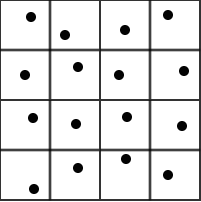
\includegraphics[width=0.5\textwidth, center]{stratified_sampling}
  \caption{Illustration of how samples are distributed within a pixel in 
  stratified sampling}
  \label{fig:image1}
\end{figure}

Stratified sampling different from uniform sampling and jittered 
sampling (see Figure~\ref{fig:image2}). Stratified sampling is preferred over 
both uniform and jittered sampling since uniform sampling can not minimize the 
effects of regular artifacts since sampling is done at regular intervals within 
the pixels and jittered sampling has the problem of introducing clumping of 
samples in one area within the pixel.

\begin{figure}[ht]
\begin{subfigure}{0.5\textwidth}
  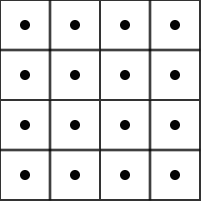
\includegraphics[width=0.5\linewidth, center]{uniform_sampling}
  \caption{Uniform Super-Sampling}
  \label{fig:subim1}
\end{subfigure}
\begin{subfigure}{0.5\textwidth}
  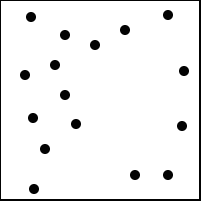
\includegraphics[width=0.5\linewidth, center]{jittered_sampling}
  \caption{Jittered Super-Sampling}
  \label{fig:subim2}
\end{subfigure}
\caption{Diagrams illustrating how samples are distributed within a pixel for
the uniform and jittered sampling methods}
\label{fig:image2}
\end{figure}


%*******************************************************
% Texture Mapping
%*******************************************************
\section{Texture Mapping}

Texture mapping is enabled by setting a texture image to a
\verb|GeometryNode|. This can be done with the following Lua command:
\begin{lstlisting}
  set_texture(<filename>)
\end{lstlisting}
This command sets the texture image on the \verb|PhongMaterial| attached to the
\verb|GeometryNode|. 

Texture mapping is implemented by generating $uv$ texture coordinates for each
of the primitives on an intersection. The texture coordinates are then used to
index into the texture map to produce a diffuse colour to be applied to the
intersection point in the lighting calculations. The following subsections
describe the $uv$ generation methods for each of the primitives and the texture
map sampling algorithm.

\subsection{Generating $uv$ Texture Coordinates}

The $uv$ texture coordinates are 2D coordinates with each coordinate having a
value in the range $[0, 1]$. This section will describe how these coordinates
are generated for each of the primitives.

\subsubsection*{Cone}
The texture coordinates for the cone primitive are calculated as follows:
\begin{equation}
\end{split}
  u &= \frac{acos(Q \cdot \begin{bmatrix} 1.0 & 0.0 & 0.0 \end{bmatrix}^{T})}
  {\pi} \\
  v &= \frac{Q_{z}}{h}
\end{split}
\end{equation}
Where $Q$ is the intersection point on the cone and $h$ is the height of the
cone. Essentially, the $u$ coordinate is the angle of rotation of the vector 
(from the origin to the intersection point) about the $z$-axis divided by $\pi$ 
in order to scale it to the range $[0, 1]$. The $v$ coordinate is calculated by
dividing the $z$ coordinate of the intersection point by the height (since the
cone is aligned along the $z$-axis).

\subsubsection*{Cylinder}
The texture coordinates for the cylinder primitive are generated in a similar
fashion as the cone:
\begin{equation}
\begin{split}
  u &= \frac{acos(\begin{bmatrix} Q_{x} & Q_{y} & 0.0 \end{bmatrix|^{T} \cdot 
  \begin{bmatrix} 1.0 & 0.0 & 0.0 \end{bmatrix}^{T})}{\pi} \\
  v &= \frac{Q_{z}}{h} + 0.5
\end{split}
\end{equation}
Note that the finite cyclinder is defined over $\frac{-h}{2} < z < \frac{h}{2}$,
thus it is necessary to add the $0.5$ term to the $v$ coordinate in order to
produce a value in the range of $[0, 1]$.

\subsubsection*{Disc}
Since the disc lies on the $xy$-plane, the texture coordinates are generated
with the following equation:
\begin{equation}
\begin{split}
  u &= \frac{Q_{x}}{2r} + 0.5 \\
  v &= \frac{Q_{y}}{2r} + 0.5 \\
\end{split}
\end{equation}
Where $r$ is the radius of the disc. The $0.5$ term is added to each coordinate 
since the diameter of the disc ranges from $[-r, r]$.

\subsubsection*{Plane}
Since the bounded plane lies on the $xz$-plane, the texture coordinates are
generated as follows:
\begin{equation}
\begin{split}
  u &= \frac{Q_{x}}{s} + 0.5 \\
  v &= \frac{Q_{z}}{s} + 0.5 
\end{split}
\end{equation}
Where $s$ is the dimension of the plane (width and height are equal). 

\subsubsection*{Torus}
To find the $uv$ coordinates for the torus we first need to define two angles.
\begin{equation}
\begin{split}
  \theta &= asin(\frac{Q_{z}}{r}) \\
  \phi &= asin(\frac{Q_{y}}{R + rcos(\theta)})
\end{split}
\end{equation}
Where $r_{0}$ is the major radius and $r_{1}$ is the minor radius. The geometric
representation of the angles are given in Figure~\ref{fig:image3}. Essentially,
$\theta$ is the angle around the tube of the vector from the center of the 
torus' tube to the intersection point. The angle $\phi$ is the radial angle of
the vector from the origin to the intersection point.

\begin{figure}[ht]
  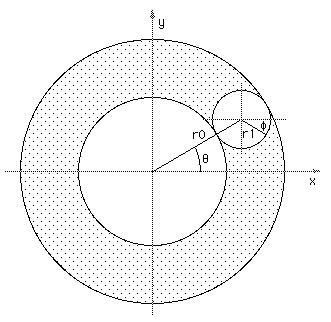
\includegraphics[width=0.5*\textwidth, center]{torus}
  \caption{Illustration of the geometric meaning of the angles \theta and \phi}
  \label{fig:image3}
\end{figure}

Using the two angles we can then generate the $uv$ coordinates as follows:
\begin{equation}
\begin{split}
  u &= \frac{\phi}{\pi} + 0.5 \\
  v &= \frac{\theta}{\pi} + 0.5
\end{split}
\end{equation}

\subsection{Sampling the Texture Map}
Once the $uv$ coordinates are generated, they are used to index into the texture
map to retrieve a colour value:
\begin{equation}
\begin{split}
  i &= \floor*{u(w - 1)} \\
  j &= \floor*{v(h - 1)}
\end{split}
\end{equation}
Where $w$ and $h$ are the width and height of texture map, respectively.

However, this does not produce very nice images since the $uv$ coordinates may
in fact index in between pixels in the texture map. A simple method to solve
this issue is to use bilinear filtering (Blinn \& Newell, 1976). The idea is to
take a weighted average of the surrounding four pixels of the texture coordinate
(Figure~\ref{fig:image4}). The closer the texture coordinate is to a pixel in
the texture map, the larger the weight of that pixel on the final colour.

\begin{figure}[ht]
  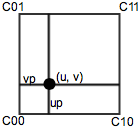
\includegraphics[width=0.5*\textwidth, center]{bilinear_filtering}
  \caption{$C_{00}$, $C_{01}$, $C_{10}$, $C_{11}$ represent the colour of the
  surrounding pixels. The area of the four rectangles created by the $uv$ 
  texture coordinate are used as the weights for the colour values.}
  \label{fig:image4}
\end{figure}

Thus, the colour, $C$, can be calculated using bilinear filtering as follows:
\begin{equation}
\begin{split}
  u_{p} = u(w - 1) - i \\
  v_{p} = v(h - 1) - j \\
  C = (1 - u_{p})(1 - v{p})C_{00} + (1 - u_{p})(v_{p})C_{01} + (u_{p})(1 -
  v_{p})C_{10} + (u_{p})(v_{p})C_{11}
\end{split}
\end{equation}


%*******************************************************
% Bump Mapping
%*******************************************************
\section{Bump Mapping}

Bump mapping is enabled by setting a bump map to a \verb|GeometryNode|. This can
be done with the following Lua command:
\begin{lstlisting}
  set_bumpmap(<filename>)
\end{lstlisting}
This command sets the bump map on the \verb|PhongMaterial| attached to the
\verb|GeometryNode|.

Bump mapping is implemented in a similiar manner as texture mapping. For each
intersection point the $uv$ coordinates of that point are generated. The $uv$
coordinates are then used to index into the bump map and sample a value
using bilinear filtering. This value is then used in the calculations to
displace the surface normal and simulate bumps on the surface of a primitive.

In order to perform the bump mapping calculations, surface tangent vectors at
the point of intersection need to be generated. For this project, these tangent
vectors were only generated for the sphere, cube and plane primitives. Thus,
bump mapping is only supported for those aforementioned primitives.

The following subsections describe how the surface tangent vectors are generated
and the calculations to perform the displacement on the surface normal.

\subsection{Generating the Tangent Vectors}
A surface can be defined in terms of three bivariate functions:
\begin{equation}
\begin{split}
  x &= x(u, v) \\
  y &= y(u, v) \\
  z &= z(u, v) \\
\end{split}
\end{equation}
Taking the partial derivatives of these functions shall give us the tangent
vectors $\vec{P_{u}}$ and $\vec{P_{v}}$ \cite{1_blinn_1978}.

\subsubsection*{Sphere}
A point on the surface of the sphere can be defined in terms of the spherical
coordinates:
\begin{equation}
\begin{split}
  x &= rcos(\theta)sin(\theta) \\
  y &= -rcos(\phi) \\
  z &= -rsin(\theta)sin(\phi) \\
\end{split}
\end{equation}
Where $\theta$ and $\phi$ can be calculated as follows:
\begin{equation}
\begin{split}
  \theta &= atan(\frac{-Q_{z}}{Q_{x}}) \\
  \phi &= acos(\frac{-Q_{y}}{r})
\end{split}
\end{equation}
$Q$ is the intersection point and $r$ is the radius of the sphere.

Taking the partial derivatives of the bivariate functions, we have:
\begin{equation}
\begin{split}
  \vec{P_{u}} = \begin{bmatrix} -rsin(\theta)sin(\phi) & 0.0 & 
  -rcos(\theta)sin(\phi) \end{bmatrix}^{T} \\
  \vec{P_{v}} = \begin{bmatrix} rcos(\theta)cos(\phi) & rsin(\phi) &
  rsin(\theta)cos(\phi) \end{bmatrix}^{T}
\end{split}
\end{equation}

\subsubsection*{Cube \& Plane}
Generating the tangent vectors for the cube and plane both follow the exact same
algorithm. First the $\vec{P_{u}}$ tangent vector is generated from the surface 
normal at the intersection point using the method described in 
\cite{6_hughes_möller_2005}. Then $\vec{P_{v}}$ is generated by taking the 
cross product between the surface normal and $\vec{P_{u}}$.

\subsection{Calculating the Displacement Vector}
Once the tangent vectors and $uv$ coordinates are generated, they are used to
calculate the displacement vector, $\vec{D}$.

First the derivatives of the bump map at the specified texture coordinate is
calculated using the finite difference method:
\begin{equation}
\begin{split}
  f_{u} = \frac{(bumpmap(u + \epsilon, v) - bumpmap(u - \epsilon, v))}
  {2\epsilon} \\
  f_{v} = \frac{(bumpmap(u, v + \epsilon) - bumpmap(u, v + \epsilon))}
  {2\epsilon}
\end{split}
\end{equation}
Where $\epsilon$ is a very small number and $bumpmap$ is a function which
samples the bump map at the specified texture coordinate using bilinear
filtering. In the \verb|C++| code the \verb|std::numeric_limits::epsilon()| 
function is used as the $\epsilon$ value.

The displacement vector can now be calculated:
\begin{equation}
\begin{split}
  \vec{D} = \frac{f_{u}(\vec{N}\times\vec{P_{v}}) -
  f_{v}(\vec{N}\times\vec{P_{u}})}{||\vec{N}||}
\end{split}
\end{equation}
Where $\vec{N}$ is the surface normal.

Now the displacement vector can be added to the normal vector to produced the
new displaced normal vector which can then be used in the lighting calculations.


%*******************************************************
% Refraction
%*******************************************************
\section{Refraction}
%*******************************************************
% Phong Shading
%*******************************************************
\section{Phong Shading}

Phong shading of meshes is supported with the new Lua command:
\begin{lstlisting}
  gr.tri_mesh(<name>, <verts>, <faces>)
\end{lstlisting}
This command differs from the \verb|gr.mesh| command in that it subdivides the
faces into triangles and generates per-vertex normals on instantiation.

The following subsections describe the triangulation and normal generation
algorithms as well as the ray-triangle intersection and normal interpolation
algorithms. 

\subsection{Face Triangulation}
Triangulating the faces is a simple matter of looping through the faces and then
splitting the face into a triangle fan. The pseudocode of the algorithm is shown
below. A face is defined as holding an array of integers which are indices into
the vertex array.

\begin{lstlisting}[caption={Mesh face triangulation}]
  function triangulate(face_list):
    new_face_list = {}
    for each face in face_list:
      v0 = face[0];
      for i = 2 to face.size():
        new_face_list.append(face(v0, face[i-1], face[i]))
      end
    end
  end
\end{lstlisting}

\subsection{Per-Vertex Normal Generation}
Generating normals per-vertex is done by calculating the normals of each face
and then adding the normal to each of the vertices connecting the face. The
normals are then normalized to produce an averaged normal for each vertex. The
algorithm is shown in the below.

\begin{lstlisting}[caption={Generating per-vertex normals}]
  function generate_normals(face_list, vert_list):
    normal_list = {}
    for each face in face_list:
      normal = (face[1] - face[0]).cross(face[2] - face[0])
      for each index in face_list:
        normal_list[index] = normal_list[index] + normal
      end
    end

    for each normal in normal_list:
      normal.normalized()
    end
  end
\end{lstlisting}

\subsection{Ray-Triangle Intersection \& Normal Interpolation}
A triangle can be defined parametrically by:
\begin{equation}
\begin{split}
  f(u, v) &= wV_{0} + uV_{1} + vV_{2} \\
  w &= 1 - u - v
\end{split}
\end{equation}
The equation can be solved for $u$, $v$, and $w$ using the algorithm described
in \cite{8_moller_trumbore_1997}.

Using the parametric values of $u$, $v$, and $w$ a normal can be determined by
taking the weighted average of the surrounding vertex normals:
\begin{equation}
  \vec{N} = wN_{0} + uN_{1} + vN_{2}
\end{equation}


%*******************************************************
% Glossy Reflections
%*******************************************************
\section{Glossy Reflections}

Glossy reflections can be enabled by setting the optional 
\newline \verb|<glossy_samples| parameter in the 
\verb|gr.render| Lua command.

Glossy reflections are implemented by perturbing the reflection ray to a random
point inside of a rectangle defined with a normal in the same direction as the
unperturbed reflection ray, $\vec{r}$ and centered at the point $r$ 
\cite{12_shirley_marschner_2009}. Many of these reflection rays are cast per 
pixel as defined by \verb|glossy_samples| parameter.

Thus, the following values must be calculated:
\begin{equation}
\begin{split}
  i = \frac{a}{2} + \zeta_{0}a \\
  j = \frac{a}{2} + \zeta_{1}a
\end{split}
\end{equation}
Where $a$ is the glossiness value and is calculated by $a = \frac{1}{1 + n_{s}}$
and $n_{s}$ is the Phong specular exponent. $\zeta_{0}$ and $\zeta_{1}$ are
uniform random numbers in the range $[0, 1]$.

These values are then used to calculate the perturbed reflection ray:
\begin{equation}
  \vec{r} = r + i\vec{U} + j\vec{V}
\end{equation}
Where $\vec{U}$ and $\vec{V}$ are orthogonal vectors in the plane of the
$a\times a$ rectangle centered at $r$. These vectors can be generated using the
algorithm described in \cite{6_hughes_moller_2005} where the normal vector is
simply in the direction of the unperturbed reflection ray.


%*******************************************************
% Perlin Noise
%*******************************************************
\section{Perlin Noise}

Perlin noise can be enabled with the following Lua command:
\begin{lstlisting}
  set_perlin(<type>)
\end{lstlisting}
This sets the perlin texture on the \verb|PhongMaterial| for the specified 
\verb|GeometryNode|.

The Perlin noise algorithm is implemented exactly as described in
\cite{11_perlin_2002}. The noise function follows the reference implementation 
as closely as possibly.

The noise function takes in as input 3D coordinates and produces a floating
point value in the range $[0, 1]$. The algorithm requires that a hash table is
initialized with random variables in order to function properly. The
\verb|Perlin::init()| function is used to initialize this hash table at the
beginning of program execution.

The noise algorithm is performed by using the coordinates of the 3D point to 
retrieve values from the hash table which are in turn used to retrieve the 
gradient vectors of the eight cube corners of the unit integer lattice . The dot 
product of the gradient vectors are then taken with each of the eight unit cube 
corners specified by the given 3D point. These "influence" values are then
trilinearly interpolated using  the three splined interpolation values 
calculated using the fractional components of the 3D coordinates. 

The \verb|Perlin| class also implements three other static functions which
produce natural textures. The \verb|Perlin::marble| function produces marble
like textures. The \verb|Perlin::cloud| function produces cloud like textures
and the \verb|Perlin::wood| function produces wood like textures. These
functions implement algorithms found in \cite{7_kora_2007}. 



%*******************************************************
% Extra Primitives
%*******************************************************
\section{Extra Primitives}

This section will described how the \verb|intersection| method was
implemented for each of the extra primitives. As mentioned in the 
previous section, the primtive classes were added to the \verb|primitives.cpp| 
source file.

The \verb|intersection| method takes two parameters. The first parameter is a
\verb|Ray| object and the second parameter is an \verb|Intersection| object. The 
intersection object is modified by an intersection method when an intersection 
has occurred. The method returns true on intersection and false otherwise.

A ray can be represented by the equation $R = O + t\vec{D}$ where
O is the ray's origin and $\vec{D}$ is the ray's direction. The \verb|Ray| 
object contains the ray's origin and direction. The point, $R$, on the ray can 
be determined given the $t$ parameter. The intersection code aims to calculate 
the value of the $t$ parameter such that the point on the ray's line is the 
point of intersection on the primitive \cite{5_drakos_1997}. 

The \verb|Intersection| object is where the intersection details are
stored such as the point of intersection, the normal at the point of
intersection (used for lighting calculations), the material of the primitive
(used for lighting calculations), the texture coordinates (used in texture
mapping), and the tangent vectors (used in bump mapping). All intersection tests 
are done in the primtives' local coordinate system with unit sized primitives.

\subsection*{Cone}
The \verb|gr.cone(<name>)| Lua command is used to create a single-ended cone 
aligned along the $z$-axis with unit height, $h$.

The cone primitive is specified by the implicit equation $x^2 + y^2 = z^2, -h <
z < h$.

In order to determine the intersection of a ray with a cone the implicit
equation must be solved by substituting in the equation of the ray:
\begin{equation}
  (O_{x} + t\vec{D}_{x})^2 + (O_{y} + t\vec{D}_{y})^2 = \\
  (O_{z} + t\vec{D}_{z})^2
\end{equation}
This equation expands to:
\begin{equation}
\begin{split}
  (\vec{D}_{x}^2 + \vec{D}_{y}^2 - \vec{D}_{z}^2)t^2 + (2O_{x}\vec{D}_{x} + 
  2O_{y}\vec{D}_{y} - 2O_{z}\vec{D}_{z})t + \\
  (O_{x}^2 + O_{y}^2 - O_{z}^2) &= 0\label{cone2}
\end{split}
\end{equation}
The equation specified in~(\ref{cone2}) can be solved for $t$ using the
quadratic equation. If the value of $t$ cannot be determined or the if $t$ is
negative, indicating that the intersection point is behind the ray's origin,
then there is no intersection. If $t$ is positive then the ray intersects the
cone and the intersection point is checked to make sure that the inequality $-h
< z < h$ is satisfied.

The normal vector is calculated by the following equation:
\begin{equation}
  \vec{N} = \begin{bmatrix} 2Q_{x} & 2Q_{y} & -2Q_{z}
  \end{bmatrix}^{T}
\end{equation}
Where $Q$ is the intersection point. The equation is essentially calculating the
gradient of the intersection point over the surface of the cone.

\subsection*{Cylinder}
The \verb|gr.cylinder(<name>)| Lua command is used to create a cylinder aligned
along the $z$-axis with unit height, $h$, and unit radius, $r$.

The cylinder primitive is specified by the implicit equation $x^2 + y^2 = r^2 =
1, \frac{-h}{2} < z < \frac{h}{2}$.

Similar to the cone, the intersection of a ray with a cylinder can be determined
by solving a quadratic equation with the following coefficients:
\begin{equation}
\begin{split}
  a_{2} &= \vec{D}_{x}^2 + \vec{D}_{y}^2 \\
  a_{1} &= 2O_{x}\vec{D}_{x} + 2O_{y}\vec{D}_{y} \\
  a_{0} &= O_{x}^2 + O_{y}^2 - 1
\end{split}
\end{equation}
The intersection of the ray with the end caps of the cylinder are determined by
testing intersection between the ray and a disc which is described later in this
section.

The normal vector is easily determined. It is essentially the vector from the
origin to the intersection point with the $z$ coordinate set to zero.

\subsection*{Disc}
The \verb|gr.disc(<name>)| Lua command is used to create a disc centered at the
origin and lying on the $xy$-plane with unit radius, $r$.

To determine the intersection of the ray with the disc, it is a simple matter of
determining if the ray intersects the plane that contains the disc and then
validating whether the intersection point lies within the disc's area. The
ray-plane intersection is described later in this section. To validate whether
the intersection point is within the disc's area, the following inequality must
be satisfied:
\begin{equation}
  Q\cdot Q \leq r^2
\end{equation}
Where $Q$ is the vector from the origin to the intersection vector.

Since the disc lies on the $xy$-plane, the normal vector is simply \newline
$\begin{bmatrix} 0.0 & 0.0 & 1.0
\end{bmatrix}^{T}$.

\subsection*{Plane}
The \verb|gr.plane(<name>)| Lua command is used to create a bounded plane 
centered at the origin and lying on the $xz$-plane with unit height, $h$, and 
width, $w$. In reality, this primitive isn't really a plane but a rectangle
(unit square). However, it can be scaled to larger size. This primitive was
added since it provides a more efficient way for modelling walls or ground in a
scene.

A point $Q$ on a plane can be found with the following equation:
\begin{equation}
  \vec{N}\cdot (Q - P) = 0
\end{equation}
Where $\vec{N}$ is the normal vector of the plane and $P$ is a known point on
the plane. To solve for $Q$ we must substitute the equation of the ray into the
plane equation which we can then solve for $t$:
\begin{equation}
  t = \frac{\vec{N}\cdot (P - O)}{\vec{N}\cdot \vec{D}}
\end{equation}
Once the intersection point is found, it is a simple matter of determining if
the intersection point is within the bounded plane. This is done by simply
validating whether the $x$ and $z$ coordinates are within the unit square.

Since the bounded plane lies on the $xz$-plane, the normal vector is simply
$\begin{bmatrix} 0.0 & 1.0 & 0.0
\end{bmatrix}^{T}$.

\subsection*{Torus}
The \verb|gr.torus(<name>)| Lua command is used to create a torus centered at
the origin and lying on the $xy$-plane with unit major radius, $R$, and a minor 
radius, $r = 0.5$.

The implementation of the ray-torus intersection test is a bit more involved
than the other primitives as it requires solving a quartic equation. The
coefficients for this quartic equation are given by \cite{13_wagner_2004}:
\begin{equation}
\begin{split}
  a_{4} &= \vec{D}\cdot\vec{D} \\
  a_{3} &= 4(\vec{D}\cdot\vec{D})(\vec{O}\cdot\vec{D}) \\
  a_{2} &= 4(\vec{O}\cdot\vec{D})^2 + 2(\vec{D}\cdot\vec{D})((\vec{O}\cdot
  \vec{O}) - r^2 - R^2) + 4R^2\vec{D}_{z}^2 \\
  a_{1} &= 4(\vec{O}\cdot\vec{D})((\vec{O}\cdot\vec{D}) - r^2 - R^2) +8R^2
  \vec{O}_{z}\vec{D}_{z} \\
  a_{0} &= ((\vec{O}\cdot\vec{O}) - r^2 - R^2)^2 + 4R^2\vec{O}_{z}^2 - 4R^2r^2
\end{split}
\end{equation}
In the intersection method, many of the terms have been computed once and
assigned to a variable so as to minimize computational overhead.

The normal vector, $\vec{N}$, at the surface of the intersection point is 
determined by taking the gradient of the implicit equation, $f$, at the 
intersection point:
\begin{equation}
\begin{split}
  \vec{N} &= \begin{bmatrix} \frac{\delta f}{\delta x} & \frac{\delta f}{\delta
  y} & \frac{\delta f}{\delta z}
  \end{bmatrix}^{T} \\
  \frac{\delta f}{\delta x} &= 4x(x^2 + y^2 + z^2 - r^2 - R^2) \\
  \frac{\delta f}{\delta y} &= 4y(x^2 + y^2 + z^2 - r^2 - R^2) \\
  \frac{\delta f}{\delta z} &= 4z(x^2 + y^2 + z^2 - r^2 - R^2) + 8R^2z
\end{split}
\end{equation}
Then solving the gradient by substituting:
\begin{equation}
\begin{split}
  x = Q_{x} \\
  y = Q_{y} \\
  z = Q_{z}
\end{split}
\end{equation}
Where $Q$ is the intersection point.


%*******************************************************
% Constructive Solid Geometry
%*******************************************************
\section{Constructive Solid Geometry}
%*******************************************************
% Soft Shadows
%*******************************************************
\section{Soft Shadows}

To enable soft shadows, the scene must contain area lights. The following Lua 
command creates an area light:
\begin{lstlisting}
  gr.disc_light(<position>, <colour>, 
  <attenuation>, <normal>, <radius>)
\end{lstlisting}
  
An optional \verb|<shadow_samples>| parameter was added to the \newline
\verb|gr.render| Lua commmand to support soft shadows. The parameter specifies 
the number of shadow rays to be cast when performing lighting calculations on 
an intersection point.

Soft shadows were implemented by randomly selecting a point on the disc light
and then casting a shadow ray from the intersection point to the point on the
disc light. The quality of the soft shadows increases as the number of shadow
rays that are cast increases (Shirley \& Marschner, 2009).

The algorithm to select the random point on the disc light is implemented by
randomly generating a rotation angle and scaling factor. The rotation angle is
used to rotate a vector on the plane of the disc light and the scaling factor is 
used to scale the vector to a length between $[0, <radius>]$. Adding the 
resultant vector to the position of the disc light produces a point on the disc
light. The method to generate a vector coincident with a plane given the normal
of the plane is described in (Hughes \& M{\"o}ller, 2005).


%*******************************************************
% Anti-Aliasing
%*******************************************************
\section{Anti-Aliasing}

To support anti-aliasing the optional \verb|<aa_samples>| parameter was added to
the \verb|gr.render| Lua command.

The parameter specifies the number of rays to cast per pixel. By default this
parameter is set to one.

Anti-aliasing is implemented using stratified super-sampling where the pixel is
divided into a $n\times n$ grid and a ray is cast from a random point within 
each grid box as shown in Figure~\ref{fig:image1}.

\begin{figure}[ht]
  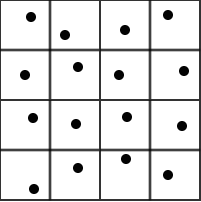
\includegraphics[width=0.5\textwidth, center]{stratified_sampling}
  \caption{Illustration of how samples are distributed within a pixel in 
  stratified sampling}
  \label{fig:image1}
\end{figure}

Stratified sampling different from uniform sampling and jittered 
sampling (see Figure~\ref{fig:image2}). Stratified sampling is preferred over 
both uniform and jittered sampling since uniform sampling can not minimize the 
effects of regular artifacts since sampling is done at regular intervals within 
the pixels and jittered sampling has the problem of introducing clumping of 
samples in one area within the pixel.

\begin{figure}[ht]
\begin{subfigure}{0.5\textwidth}
  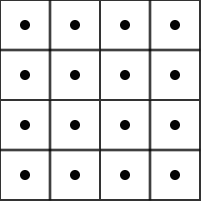
\includegraphics[width=0.5\linewidth, center]{uniform_sampling}
  \caption{Uniform Super-Sampling}
  \label{fig:subim1}
\end{subfigure}
\begin{subfigure}{0.5\textwidth}
  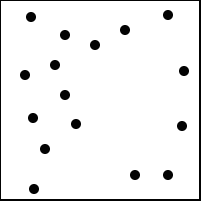
\includegraphics[width=0.5\linewidth, center]{jittered_sampling}
  \caption{Jittered Super-Sampling}
  \label{fig:subim2}
\end{subfigure}
\caption{Diagrams illustrating how samples are distributed within a pixel for
the uniform and jittered sampling methods}
\label{fig:image2}
\end{figure}


%*******************************************************
% Texture Mapping
%*******************************************************
\section{Texture Mapping}

Texture mapping is enabled by setting a texture image to a
\verb|GeometryNode|. This can be done with the following Lua command:
\begin{lstlisting}
  set_texture(<filename>)
\end{lstlisting}
This command sets the texture image on the \verb|PhongMaterial| attached to the
\verb|GeometryNode|. 

Texture mapping is implemented by generating $uv$ texture coordinates for each
of the primitives on an intersection. The texture coordinates are then used to
index into the texture map to produce a diffuse colour to be applied to the
intersection point in the lighting calculations. The following subsections
describe the $uv$ generation methods for each of the primitives and the texture
map sampling algorithm.

\subsection{Generating $uv$ Texture Coordinates}

The $uv$ texture coordinates are 2D coordinates with each coordinate having a
value in the range $[0, 1]$. This section will describe how these coordinates
are generated for each of the primitives.

\subsubsection*{Cone}
The texture coordinates for the cone primitive are calculated as follows:
\begin{equation}
\end{split}
  u &= \frac{acos(Q \cdot \begin{bmatrix} 1.0 & 0.0 & 0.0 \end{bmatrix}^{T})}
  {\pi} \\
  v &= \frac{Q_{z}}{h}
\end{split}
\end{equation}
Where $Q$ is the intersection point on the cone and $h$ is the height of the
cone. Essentially, the $u$ coordinate is the angle of rotation of the vector 
(from the origin to the intersection point) about the $z$-axis divided by $\pi$ 
in order to scale it to the range $[0, 1]$. The $v$ coordinate is calculated by
dividing the $z$ coordinate of the intersection point by the height (since the
cone is aligned along the $z$-axis).

\subsubsection*{Cylinder}
The texture coordinates for the cylinder primitive are generated in a similar
fashion as the cone:
\begin{equation}
\begin{split}
  u &= \frac{acos(\begin{bmatrix} Q_{x} & Q_{y} & 0.0 \end{bmatrix|^{T} \cdot 
  \begin{bmatrix} 1.0 & 0.0 & 0.0 \end{bmatrix}^{T})}{\pi} \\
  v &= \frac{Q_{z}}{h} + 0.5
\end{split}
\end{equation}
Note that the finite cyclinder is defined over $\frac{-h}{2} < z < \frac{h}{2}$,
thus it is necessary to add the $0.5$ term to the $v$ coordinate in order to
produce a value in the range of $[0, 1]$.

\subsubsection*{Disc}
Since the disc lies on the $xy$-plane, the texture coordinates are generated
with the following equation:
\begin{equation}
\begin{split}
  u &= \frac{Q_{x}}{2r} + 0.5 \\
  v &= \frac{Q_{y}}{2r} + 0.5 \\
\end{split}
\end{equation}
Where $r$ is the radius of the disc. The $0.5$ term is added to each coordinate 
since the diameter of the disc ranges from $[-r, r]$.

\subsubsection*{Plane}
Since the bounded plane lies on the $xz$-plane, the texture coordinates are
generated as follows:
\begin{equation}
\begin{split}
  u &= \frac{Q_{x}}{s} + 0.5 \\
  v &= \frac{Q_{z}}{s} + 0.5 
\end{split}
\end{equation}
Where $s$ is the dimension of the plane (width and height are equal). 

\subsubsection*{Torus}
To find the $uv$ coordinates for the torus we first need to define two angles.
\begin{equation}
\begin{split}
  \theta &= asin(\frac{Q_{z}}{r}) \\
  \phi &= asin(\frac{Q_{y}}{R + rcos(\theta)})
\end{split}
\end{equation}
Where $r_{0}$ is the major radius and $r_{1}$ is the minor radius. The geometric
representation of the angles are given in Figure~\ref{fig:image3}. Essentially,
$\theta$ is the angle around the tube of the vector from the center of the 
torus' tube to the intersection point. The angle $\phi$ is the radial angle of
the vector from the origin to the intersection point.

\begin{figure}[ht]
  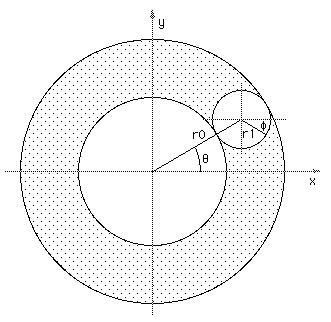
\includegraphics[width=0.5*\textwidth, center]{torus}
  \caption{Illustration of the geometric meaning of the angles \theta and \phi}
  \label{fig:image3}
\end{figure}

Using the two angles we can then generate the $uv$ coordinates as follows:
\begin{equation}
\begin{split}
  u &= \frac{\phi}{\pi} + 0.5 \\
  v &= \frac{\theta}{\pi} + 0.5
\end{split}
\end{equation}

\subsection{Sampling the Texture Map}
Once the $uv$ coordinates are generated, they are used to index into the texture
map to retrieve a colour value:
\begin{equation}
\begin{split}
  i &= \floor*{u(w - 1)} \\
  j &= \floor*{v(h - 1)}
\end{split}
\end{equation}
Where $w$ and $h$ are the width and height of texture map, respectively.

However, this does not produce very nice images since the $uv$ coordinates may
in fact index in between pixels in the texture map. A simple method to solve
this issue is to use bilinear filtering (Blinn \& Newell, 1976). The idea is to
take a weighted average of the surrounding four pixels of the texture coordinate
(Figure~\ref{fig:image4}). The closer the texture coordinate is to a pixel in
the texture map, the larger the weight of that pixel on the final colour.

\begin{figure}[ht]
  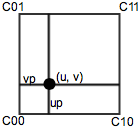
\includegraphics[width=0.5*\textwidth, center]{bilinear_filtering}
  \caption{$C_{00}$, $C_{01}$, $C_{10}$, $C_{11}$ represent the colour of the
  surrounding pixels. The area of the four rectangles created by the $uv$ 
  texture coordinate are used as the weights for the colour values.}
  \label{fig:image4}
\end{figure}

Thus, the colour, $C$, can be calculated using bilinear filtering as follows:
\begin{equation}
\begin{split}
  u_{p} = u(w - 1) - i \\
  v_{p} = v(h - 1) - j \\
  C = (1 - u_{p})(1 - v{p})C_{00} + (1 - u_{p})(v_{p})C_{01} + (u_{p})(1 -
  v_{p})C_{10} + (u_{p})(v_{p})C_{11}
\end{split}
\end{equation}


%*******************************************************
% Bump Mapping
%*******************************************************
\section{Bump Mapping}

Bump mapping is enabled by setting a bump map to a \verb|GeometryNode|. This can
be done with the following Lua command:
\begin{lstlisting}
  set_bumpmap(<filename>)
\end{lstlisting}
This command sets the bump map on the \verb|PhongMaterial| attached to the
\verb|GeometryNode|.

Bump mapping is implemented in a similiar manner as texture mapping. For each
intersection point the $uv$ coordinates of that point are generated. The $uv$
coordinates are then used to index into the bump map and sample a value
using bilinear filtering. This value is then used in the calculations to
displace the surface normal and simulate bumps on the surface of a primitive.

In order to perform the bump mapping calculations, surface tangent vectors at
the point of intersection need to be generated. For this project, these tangent
vectors were only generated for the sphere, cube and plane primitives. Thus,
bump mapping is only supported for those aforementioned primitives.

The following subsections describe how the surface tangent vectors are generated
and the calculations to perform the displacement on the surface normal.

\subsection{Generating the Tangent Vectors}
A surface can be defined in terms of three bivariate functions:
\begin{equation}
\begin{split}
  x &= x(u, v) \\
  y &= y(u, v) \\
  z &= z(u, v) \\
\end{split}
\end{equation}
Taking the partial derivatives of these functions shall give us the tangent
vectors $\vec{P_{u}}$ and $\vec{P_{v}}$ \cite{1_blinn_1978}.

\subsubsection*{Sphere}
A point on the surface of the sphere can be defined in terms of the spherical
coordinates:
\begin{equation}
\begin{split}
  x &= rcos(\theta)sin(\theta) \\
  y &= -rcos(\phi) \\
  z &= -rsin(\theta)sin(\phi) \\
\end{split}
\end{equation}
Where $\theta$ and $\phi$ can be calculated as follows:
\begin{equation}
\begin{split}
  \theta &= atan(\frac{-Q_{z}}{Q_{x}}) \\
  \phi &= acos(\frac{-Q_{y}}{r})
\end{split}
\end{equation}
$Q$ is the intersection point and $r$ is the radius of the sphere.

Taking the partial derivatives of the bivariate functions, we have:
\begin{equation}
\begin{split}
  \vec{P_{u}} = \begin{bmatrix} -rsin(\theta)sin(\phi) & 0.0 & 
  -rcos(\theta)sin(\phi) \end{bmatrix}^{T} \\
  \vec{P_{v}} = \begin{bmatrix} rcos(\theta)cos(\phi) & rsin(\phi) &
  rsin(\theta)cos(\phi) \end{bmatrix}^{T}
\end{split}
\end{equation}

\subsubsection*{Cube \& Plane}
Generating the tangent vectors for the cube and plane both follow the exact same
algorithm. First the $\vec{P_{u}}$ tangent vector is generated from the surface 
normal at the intersection point using the method described in 
\cite{6_hughes_möller_2005}. Then $\vec{P_{v}}$ is generated by taking the 
cross product between the surface normal and $\vec{P_{u}}$.

\subsection{Calculating the Displacement Vector}
Once the tangent vectors and $uv$ coordinates are generated, they are used to
calculate the displacement vector, $\vec{D}$.

First the derivatives of the bump map at the specified texture coordinate is
calculated using the finite difference method:
\begin{equation}
\begin{split}
  f_{u} = \frac{(bumpmap(u + \epsilon, v) - bumpmap(u - \epsilon, v))}
  {2\epsilon} \\
  f_{v} = \frac{(bumpmap(u, v + \epsilon) - bumpmap(u, v + \epsilon))}
  {2\epsilon}
\end{split}
\end{equation}
Where $\epsilon$ is a very small number and $bumpmap$ is a function which
samples the bump map at the specified texture coordinate using bilinear
filtering. In the \verb|C++| code the \verb|std::numeric_limits::epsilon()| 
function is used as the $\epsilon$ value.

The displacement vector can now be calculated:
\begin{equation}
\begin{split}
  \vec{D} = \frac{f_{u}(\vec{N}\times\vec{P_{v}}) -
  f_{v}(\vec{N}\times\vec{P_{u}})}{||\vec{N}||}
\end{split}
\end{equation}
Where $\vec{N}$ is the surface normal.

Now the displacement vector can be added to the normal vector to produced the
new displaced normal vector which can then be used in the lighting calculations.


%*******************************************************
% Refraction
%*******************************************************
\section{Refraction}
%*******************************************************
% Phong Shading
%*******************************************************
\section{Phong Shading}

Phong shading of meshes is supported with the new Lua command:
\begin{lstlisting}
  gr.tri_mesh(<name>, <verts>, <faces>)
\end{lstlisting}
This command differs from the \verb|gr.mesh| command in that it subdivides the
faces into triangles and generates per-vertex normals on instantiation.

The following subsections describe the triangulation and normal generation
algorithms as well as the ray-triangle intersection and normal interpolation
algorithms. 

\subsection{Face Triangulation}
Triangulating the faces is a simple matter of looping through the faces and then
splitting the face into a triangle fan. The pseudocode of the algorithm is shown
below. A face is defined as holding an array of integers which are indices into
the vertex array.

\begin{lstlisting}[caption={Mesh face triangulation}]
  function triangulate(face_list):
    new_face_list = {}
    for each face in face_list:
      v0 = face[0];
      for i = 2 to face.size():
        new_face_list.append(face(v0, face[i-1], face[i]))
      end
    end
  end
\end{lstlisting}

\subsection{Per-Vertex Normal Generation}
Generating normals per-vertex is done by calculating the normals of each face
and then adding the normal to each of the vertices connecting the face. The
normals are then normalized to produce an averaged normal for each vertex. The
algorithm is shown in the below.

\begin{lstlisting}[caption={Generating per-vertex normals}]
  function generate_normals(face_list, vert_list):
    normal_list = {}
    for each face in face_list:
      normal = (face[1] - face[0]).cross(face[2] - face[0])
      for each index in face_list:
        normal_list[index] = normal_list[index] + normal
      end
    end

    for each normal in normal_list:
      normal.normalized()
    end
  end
\end{lstlisting}

\subsection{Ray-Triangle Intersection \& Normal Interpolation}
A triangle can be defined parametrically by:
\begin{equation}
\begin{split}
  f(u, v) &= wV_{0} + uV_{1} + vV_{2} \\
  w &= 1 - u - v
\end{split}
\end{equation}
The equation can be solved for $u$, $v$, and $w$ using the algorithm described
in \cite{8_moller_trumbore_1997}.

Using the parametric values of $u$, $v$, and $w$ a normal can be determined by
taking the weighted average of the surrounding vertex normals:
\begin{equation}
  \vec{N} = wN_{0} + uN_{1} + vN_{2}
\end{equation}


%*******************************************************
% Perlin Noise
%*******************************************************
\section{Perlin Noise}

Perlin noise can be enabled with the following Lua command:
\begin{lstlisting}
  set_perlin(<type>)
\end{lstlisting}
This sets the perlin texture on the \verb|PhongMaterial| for the specified 
\verb|GeometryNode|.

The Perlin noise algorithm is implemented exactly as described in
\cite{11_perlin_2002}. The noise function follows the reference implementation 
as closely as possibly.

The noise function takes in as input 3D coordinates and produces a floating
point value in the range $[0, 1]$. The algorithm requires that a hash table is
initialized with random variables in order to function properly. The
\verb|Perlin::init()| function is used to initialize this hash table at the
beginning of program execution.

The noise algorithm is performed by using the coordinates of the 3D point to 
retrieve values from the hash table which are in turn used to retrieve the 
gradient vectors of the eight cube corners of the unit integer lattice . The dot 
product of the gradient vectors are then taken with each of the eight unit cube 
corners specified by the given 3D point. These "influence" values are then
trilinearly interpolated using  the three splined interpolation values 
calculated using the fractional components of the 3D coordinates. 

The \verb|Perlin| class also implements three other static functions which
produce natural textures. The \verb|Perlin::marble| function produces marble
like textures. The \verb|Perlin::cloud| function produces cloud like textures
and the \verb|Perlin::wood| function produces wood like textures. These
functions implement algorithms found in \cite{7_kora_2007}. 


%*******************************************************
% Glossy Reflections
%*******************************************************
\section{Glossy Reflections}

Glossy reflections can be enabled by setting the optional 
\newline \verb|<glossy_samples| parameter in the 
\verb|gr.render| Lua command.

Glossy reflections are implemented by perturbing the reflection ray to a random
point inside of a rectangle defined with a normal in the same direction as the
unperturbed reflection ray, $\vec{r}$ and centered at the point $r$ 
\cite{12_shirley_marschner_2009}. Many of these reflection rays are cast per 
pixel as defined by \verb|glossy_samples| parameter.

Thus, the following values must be calculated:
\begin{equation}
\begin{split}
  i = \frac{a}{2} + \zeta_{0}a \\
  j = \frac{a}{2} + \zeta_{1}a
\end{split}
\end{equation}
Where $a$ is the glossiness value and is calculated by $a = \frac{1}{1 + n_{s}}$
and $n_{s}$ is the Phong specular exponent. $\zeta_{0}$ and $\zeta_{1}$ are
uniform random numbers in the range $[0, 1]$.

These values are then used to calculate the perturbed reflection ray:
\begin{equation}
  \vec{r} = r + i\vec{U} + j\vec{V}
\end{equation}
Where $\vec{U}$ and $\vec{V}$ are orthogonal vectors in the plane of the
$a\times a$ rectangle centered at $r$. These vectors can be generated using the
algorithm described in \cite{6_hughes_moller_2005} where the normal vector is
simply in the direction of the unperturbed reflection ray.


%*******************************************************
% Conclusion
%*******************************************************
\pdfbookmark[1]{Conclusion}{conclusion}
\chapter{Conclusion}

% Back Matter
%*******************************************************
% References
%*******************************************************
\pdfbookmark[1]{References}{references}
\addcontentsline{toc}{chapter}{References}

\bibliographystyle{unsrt}
\bibliography{references}


    
\end{document}
